%-------------------------------------------------------------------------------
\section{Problem}\label{s:problem}
%-------------------------------------------------------------------------------

On an empirical level, the problem is that Linux occasionally will run a BE
process on one core, unaware that an LC process is runnable and waiting on
another. This observation points to a problem with the \cgroups{} weight
interface: it is expensive to enforce weights across cores, which is why Linux
avoids doing so. The \cgroups{} weight interface also is not good at isolating
for another reason: it doesn't really try to. Weights are supposed to be ends of
a spectrum, and many small weights can add up.

\subsection{Empirical problem}

\begin{figure}[t]
    \centering
    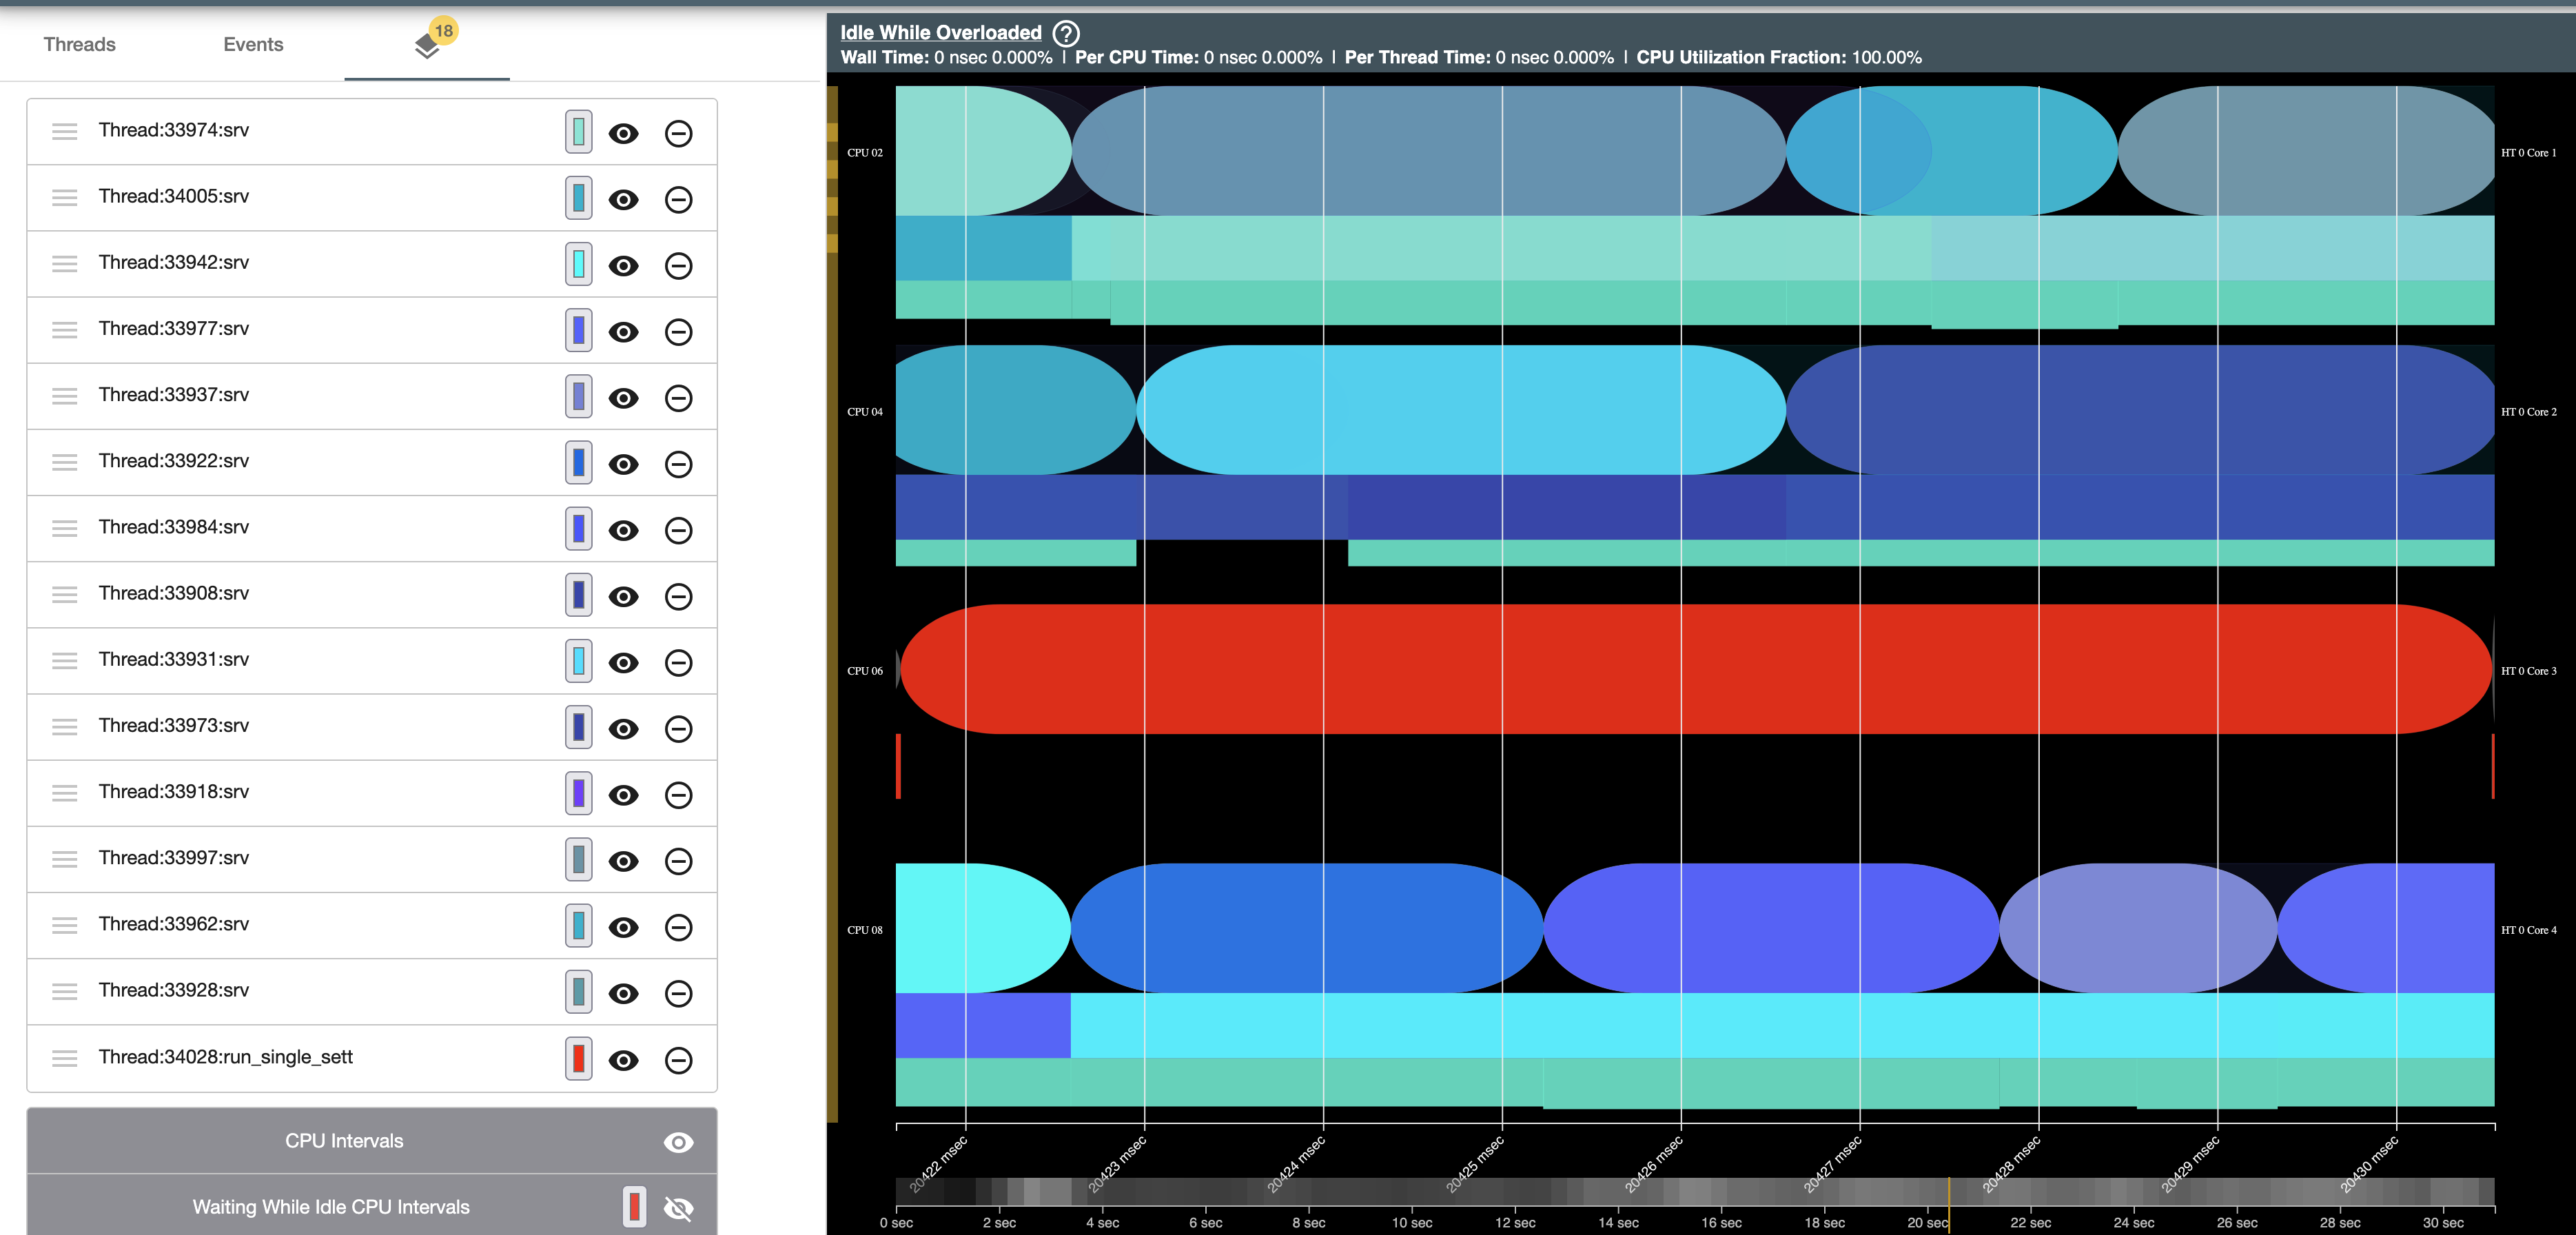
\includegraphics[width=\columnwidth]{graphs/schedviz.png}
    \caption{Each thread is a different color. Circles represent which
    thread is running on that core, while rectangles underneath show waiting but
    runnable threads
    }\label{fig:schedviz}
\end{figure}

We analyze perf traces of the scheduling decisions, and the failure mode we
observe is that \textit{one core is running a BE process, while an LC process is
waiting on another}. We visualize the trace using schedviz~\cite{TODO}; a 10ms
outtake of the resulting image is show in \autoref{fig:schedviz}. The process
running on each core is shown as a an oval, and queued processes are shown as
rectangles below. The root of the undesirable behavior is clear: on core 6, the
red process that is running the whole time is a BE process, whereas LC threads,
shown in varying shades of blue, are queued on the other cores.

The reason this happens is that Linux maintains a separate runqueue on each
core, in order to avoid the synchronization overheads of accessing global state
for every scheduling decision. Within each runqueue, Linux does a pretty good
job of maintaining the correct ratio of received cputime; but it does not
enforce the weight ratios across cores. This leads to the above failure mode,
where one core has no runnable high weight processes and thus runs a low weight
one, whereas another core has queued high weight processes. This problem goes
away when there are no BE processes, because cores try to steal work before
going idle.

\subsection{Weights across cores}

The root of the problem goes deeper than just a poor implementation: in a
setting of per-core runqueues where synchronization is expensive, a weight-based
interface is at odds with machine-wide policy enforcement.

\begin{figure}[t]
    \centering
    
\includegraphics[width=0.8\columnwidth]{graphs/todo.png}
    \caption{the low load setting of the same experiment, running on cores
    across two NUMA nodes}\label{fig:across-numa}
\end{figure}

% what is the experiment here? more cores? cores across NUMA nodes so it
% migrates less?
We see that this is the case by running the same experiment in a setting where
synchronization is even more expensive: on cores across NUMA nodes. In
\autoref{fig:across-numa}, we run the exact same experiment, but use cores that
span different NUMA nodes. The graph shows a greatly increased latency spike,
due to a decreased number of migrations: in the original experiment there were
XX migrations over the course of the experiment, and in this version there were
only YY. This indicates that, as expected, more synchronization points increases
the degree to which the weights are enforced across cores. In order to strictly
and completely enforce the weights, the scheduler would need to synchronize at
every scheduling decision: calculating whether a given process is owed time
globally requires knowing the total weight across all cores as well as the sum
of time that all the processes in the group have gotten. 


\subsection{Weights add up}


\begin{figure}[t]
    \centering
    
\includegraphics[width=0.8\columnwidth]{graphs/todo.png}
    \caption{running the same experiment, with an increasing number of BE
    workloads}\label{fig:many-be}
\end{figure}


Although low weights run infrequently, they still get a fair share, and in doing
so impact the latency of the higher weight (LC) processes. A large number of BE
workloads each with a small weight adds up to represent a significant amount of
weight in the system, now contending directly with the LC workload. In
\autoref{fig:many-be}, we show the mean and 99th pctile latency increase when
starting different numbers of BE workload, as compared to an uncontended
baseline. As expected, as the number of BE workloads goes up, the impact on the
latency of the LC server goes up.

Weights also interact with Linux's 4ms scheduling tick granularity: when it is a
low-weight processes time to run, it will likely be scheduled for a full tick.
It is common for microservices to have SLAs in the order of 10ms or even less,
where a gap of 4ms will have a significant impact on response latency.
Compounded with a large number of BE workloads, this can lead to significant
overheads, even in a world where weights are correctly enforced across cores.




